% Created 2019-09-30 Пн 11:19
% Intended LaTeX compiler: pdflatex
\documentclass[11pt]{article}
\usepackage[utf8]{inputenc}
\usepackage[T1]{fontenc}
\usepackage{graphicx}
\usepackage{grffile}
\usepackage{longtable}
\usepackage{wrapfig}
\usepackage{rotating}
\usepackage[normalem]{ulem}
\usepackage{amsmath}
\usepackage{textcomp}
\usepackage{amssymb}
\usepackage{capt-of}
\usepackage{hyperref}
\usepackage[T2A]{fontenc}
\usepackage[a4paper,left=3cm,top=2cm,right=1.5cm,bottom=2cm,marginparsep=7pt,marginparwidth=.6in]{geometry}
\usepackage{cmap}
\usepackage{xcolor}
\usepackage{listings}
\usepackage{polyglossia}
\setdefaultlanguage{russian} \setotherlanguage{english}
\setmainfont{Liberation Serif}
\setsansfont{Liberation Sans}
\setmonofont[Contextuals=Alternate,Ligatures={TeX}]{Fira Code Regular}
\author{Крутько Никита}
\date{\today}
\title{}
\hypersetup{
 pdfauthor={Крутько Никита},
 pdftitle={},
 pdfkeywords={},
 pdfsubject={},
 pdfcreator={Emacs 26.1 (Org mode 9.1.9)}, 
 pdflang={Russian}}
\begin{document}

\thispagestyle{empty}
\large
\newfontfamily\lstcomment[Scale=0.6]{Fira Code Regular}
\newfontfamily\lstbasic[Scale=0.8,Contextuals=Alternate,Ligatures={TeX}]{Fira Code Regular}
\lstset{
  frame = shadowbox,
  commentstyle = \lstcomment\it\small,
  basicstyle = \lstbasic\small,
  numberstyle = \lstbasic\tiny,numbers=left,
  stringstyle = \lstbasic\it\small,
}
\begin{center}
\textbf{Санкт-Петербургский Национальный Исследовательский}\\
\textbf{Университет Информационных Технологий, Механики и Оптики}\\
\textbf{Факультет Программной Инженерии и Компьютерной Техники}\\
\end{center}
\vspace{1em}
\begin{center}

\includegraphics[width=120pt]{./itmo-logo.png}
\end{center}
\LARGE
\vspace{5em}
\begin{center}
\textbf{Вариант №-7}\\
\textbf{Лабораторная работа №1}\\
\Large
\textbf{по дисциплине}\\
\LARGE
\textbf{\emph{'Основы профессиональной деятельности'}}\\
\end{center}
\vspace{11em}
\large
\begin{flushright}
\textbf{Выполнил:}\\
\textbf{Студент группы P3113}\\
\textbf{\emph{Крутько Никита} : 242570}\\
\textbf{Преподаватель:}\\
\textbf{\emph{Перминов Илья Валентинович}}\\
\end{flushright}
\vspace{4em}
\large
\begin{center}
\textbf{Санкт-Петербург 2019 г.}
\end{center}
\pagebreak{}
\setcounter{tocdepth}{2}
\tableofcontents
\vspace{2em}
\section{Задание}
\label{sec:org6072d6b}
\begin{enumerate}
\item Create tree hierarchy with directory, files and its contents. Use lab0 as tree root in your home directory and following commands for tree creation: mkdir, echo, cat, touch, ls, pwd, cd, more, cp, rm, rmdir, mv.\\
\item Set up file and directory permissions chmod, using different approaches.\\
\item Copy tree parts and create links with cp and ln, as well as with cat and io streams redirection.\\
\item Using cat, wc, ls, head, tail, echo, sort, grep looks up and filters directory, files and data in it.\\
\item Remove files using rm and rmdir according following:
\end{enumerate}

\section{Листинги}
\label{sec:orgf8bbaef}
\small
\lstset{language=bash,label= ,caption={tree.sh},captionpos=b,numbers=none}
\begin{lstlisting}
#!/usr/bin/env bash
TMP_PATH=.
touch $TMP_PATH/{bibarel2,mienshao5,volcarona0}
mkdir $TMP_PATH/{fraxure4,haunter2,nuzleaf7}
# fraxure4
TMP_PATH=fraxure4
touch $TMP_PATH/quagsire
mkdir $TMP_PATH/{rhyperior,linoone,makuhita}
# haunter2
TMP_PATH=haunter2
touch $TMP_PATH/gurdur
mkdir $TMP_PATH/{yamask,snorunt,hippopotas,bellossom}
# nuzleaf7
TMP_PATH=nuzleaf7
touch $TMP_PATH/{aipom,ambipom,weavile}
mkdir $TMP_PATH/{swalot,cyndaquil}

ls -lR | awk 'BEGIN{RS="\n\n"; FS="\n";
system("rm -f .files; touch .files;\
	rm -f .dirs; touch .dirs;\
	rm -f .all; touch .all")} {
   split($1, dir, ":");
   if (NF > 2 && $NF != "") {
      for (i = 3; i <= NF; i++) {
	   split($i, f_info, " ")
	   split(f_info[1], chs, "")
	   if (chs[1] == "d") {
	      system("echo " dir[1] "/" f_info[9] " >> .dirs")
	   } else {
	      system("echo " dir[1] "/" f_info[9] " >> .files")
	   }
	   system("echo " dir[1] "/" f_info[9] " >> .all")
      }
   }
}'
\end{lstlisting}
\vspace{2em}
\lstset{language=bash,label= ,caption={setup-files.sh},captionpos=b,numbers=none}
\begin{lstlisting}
#!/usr/bin/env bash
# bibarel2:
awk '/bibarel2/{system("echo \
\"Возможности  Overland=8 Surface=9 Jump=3 Power=3\n\
Intelligence=3 Fountain=0\" > " $0)}' .files
# quagsire:
awk '/quagsire/{system("echo \
\"Способности  Tail Whip Water Gun\n\
Mud Sport Mud Shot Slam Mud Bomb Amnesia Yawn Earthquake Rain Dance\n\
Haze Mist Muddy Water\" > " $0)}' .files
# gurdurr:
awk '/gurdurr/{system("echo \
\"Ходы  Block Drain Punch Fire Punch\n\
Helping Hand Ice Punch Knock Off Low Kick Sleep Talk Snore Superpower\n\
Thunderpunch\" > " $0)}' .files
# mienshao5:
awk '/mienshao5/{system("echo \
\"satk=10 sdef=6 spd=11\" > " $0)}' .files
# aipom:
awk '/aipom/{system("echo \
\"Тип покемона\nNORMAL NONE\" > " $0)}' .files
# ambipom:
awk '/ambipom/{system("echo \
\"weight=44.8 height=47.0 atk=10\ndef=7\" > " $0)}' .files
# weavile:
awk '/weavile/{system("echo \
\"Возможности  Overland=10 Surface=6 Jump=4 Power=4\n\
Intelligence=4 Icestep=0 Stealth=0\" > " $0)}' .files
# volcarona0:
awk '/volcarona0/{system("echo \
\"Способности  Leech Life\n\
Gust Fire Spin Whirlwind Silver Wind Quiver Dance Heat Wave Bug Buzz\n\
Rage Powder Hurricane Fiery Dance\" > " $0)}' .files
\end{lstlisting}
\vspace{2em}
\lstset{language=bash,label= ,caption={permissions.sh},captionpos=b,numbers=none}
\begin{lstlisting}
#!/usr/bin/env bash
awk '/fraxure4$/{system("chmod u=rwx,g=rx,o=w " $0)}' .all
awk '/rhyperior$/{system("chmod 777 " $0)}' .all
awk '/linoone$/{system("chmod 337 " $0)}' .all
awk '/makuhita$/{system("chmod u=rwx,g=wx,o=rwx " $0)}' .all
awk '/quagsire$/{system("chmod u-rwx,g=rw,o=w " $0)}' .all
awk '/bibarel2$/{system("chmod u=rw,g=w,o=r " $0)}' .all
awk '/yamask$/{system("chmod u=wx,g=x,o=w " $0)}' .all
awk '/snorunt$/{system("chmod u=rx,g=rwx,o=rwx " $0)}' .all
awk '/hippopotas$/{system("chmod 500 " $0)}' .all
awk '/gurdurr$/{system("chmod 540 " $0)}' .all
awk '/bellossom$/{system("chmod 511 " $0)}' .all
awk '/haunter2$/{system("chmod 700 " $0)}' .all
awk '/mienshao5$/{system("chmod 640 " $0)}' .all
awk '/swalot$/{system("chmod 307 " $0)}' .all
awk '/aipom$/{system("chmod u-rwx,g=r,o=r " $0)}' .all
awk '/ambipom$/{system("chmod u-rwx,g=wx,o=w " $0)}' .all
awk '/cyndaquil$/{system("chmod u=rx,g=w,o=r " $0)}' .all
awk '/weavile$$/{system("chmod 064 " $0)}' .all
awk '/nuzleaf7$/{system("chmod u=wx,g=x,o=w " $0)}' .all
awk '/volcarona0$/{system("chmod u-rwx,g=rw,o=w " $0)}' .all
\end{lstlisting}
\vspace{2em}
\lstset{language=bash,label= ,caption={copy.sh},captionpos=b,numbers=none}
\begin{lstlisting}
#!/usr/bin/env bash
#cp -r haunter2 fraxure4/rhyperior
awk '/\.\/haunter2\//{
    split($0, vals, "/")
    "stat -c \"%A\" "$0 | getline st
    "stat -c \"%a\" "$0 | getline sts
    system("chmod u+r "$0)
    split(st, chars, "")
    system("cp -r "$0" fraxure4/rhyperior")
    if (chars[1] == "d") {
       system("echo ./fraxure4/rhyperior/" vals[3] " >> .dirs")
    } else {
       system("echo ./fraxure4/rhyperior/" vals[3] " >> .files")
    }
    system("echo ./fraxure4/rhyperior/" vals[3] " >> .all")
    system("chmod " sts " " $0 " ./fraxure4/rhyperior/" vals[3] "")
}' .all
ln -s fraxure4 Copy_52

ln -s mienshao5 ./nuzleaf7/aipommienshao

stat {nuzleaf7/weavile,fraxure4/quagsire} -c "%a %n" \
    | awk '{
	system("chmod u+r " $2)
	system("cat " $2 " >> volcarona0_66")
	system("chmod " $1 " " $2)
    }' && echo "./volcarona0_66" >> .files
cat mienshao5 > haunter2/gurdurrmienshao &&
    echo "./haunter2/gurdurrmienshao" >> .files &&
    echo "./haunter2/gurdurrmienshao" >> .all

stat {./nuzleaf7/cyndaquil,./volcarona0} -c '%a %n' \
     | tr '\n' ' ' \
     | awk '{
	 system("chmod u+w " $2 "; chmod u+r " $4)
	 system("cp " $4 " " $2 "; echo " $2 " >> .files")
	 system("chmod " $1 " " $2 "; chmod " $3 " " $4)
     }'
awk '{
    system("ln volcarona0 " $1)
    system("echo " $1 " >> .files")
}' <<< "./nuzleaf7/weavilevolcarona"
\end{lstlisting}
\vspace{2em}
\lstset{language=bash,label= ,caption={filter.sh},captionpos=b,numbers=none}
\begin{lstlisting}
#!/usr/bin/env bash
wc -l ./nuzleaf7/{aipom,ambipom,weavile} | sort -nk1
awk '/\.\/fraxure4\/.*/{
    "stat -c \"%s %a\" "$0 | getline st
    print st,$0
}' .files | sort -nrk1 | awk '{print $2 " " $3}'
awk '/^\.\/(a[^\/]*)|(.*\/a.*)$/{
    "stat -c \"%a\" "$0 | getline st
    system("chmod u+r "$0);system("cat "$0)
    system("chmod " st " " $0)
}' .files | sort
bash -c "wc -l ./volcarona0 >> ./volcarona0" 2> /tmp/krutna.err
awk '/.*qu.*/{
    "stat -c \"%s\" "$0 | getline st
    print st,$1|"sort -nrk1"
}' .files 2>/dev/null | awk '{print $2}' | tail -n3
awk '/mienshao5$/{system("cat "$0)}' .files 2>&1 | sort -n
\end{lstlisting}
\vspace{2em}
\lstset{language=bash,label= ,caption={rm.sh},captionpos=b,numbers=none}
\begin{lstlisting}
#!/usr/bin/env bash
awk '/volcarona0/{system("rm -rf " $0)}' .all
awk '/weavile/{system("rm -rf " $0)}' .all
awk '/Copy_.*/{system("rm -rf " $0)}' .all
awk '/weavilevolcaro.*/{system("rm -rf " $0)}' .all
awk '/^nuzleaf7$/{
    system("chmod -R u+rw " $0)
    system("rm -rf " $0)
}' .all
awk '/hippopotas/{system("rm -rf " $0)}' .all
\end{lstlisting}

\section{Вывод программы}
\label{sec:org6eaed8d}
\begin{verbatim}
wc: ./nuzleaf7/aipom: Отказано в доступе
wc: ./nuzleaf7/ambipom: Отказано в доступе
wc: ./nuzleaf7/weavile: Отказано в доступе
  0 итого
62 ./fraxure4/quagsire
644 ./fraxure4/rhyperior/gurdur
def=7
NORMAL NONE
weight=44.8 height=47.0 atk=10
Тип покемона
./nuzleaf7/cyndaquil
./fraxure4/quagsire
satk=10 sdef=6 spd=11
\end{verbatim}
\normalsize
\section{Вывод}
\label{sec:org57dcd44}
Я вспомнил некоторые команды UNIX, а также изучил несколько новых, таких как stat. Также познакомился с AWK и использовал его в своей работе, т.к. с его помощью многие вещи решались довольно красиво. По возможности старался писать хороший код, на который как минимум мне самому было бы приятно смотреть.
\pagebreak{}
\section{Текст заданий}
\label{sec:orge8ed9bb}
\begin{enumerate}
\item Create tree hierarchy with directory, files and its contents. Use lab0 as tree root in your home directory and following commands for tree creation: mkdir, echo, cat, touch, ls, pwd, cd, more, cp, rm, rmdir, mv.
\end{enumerate}
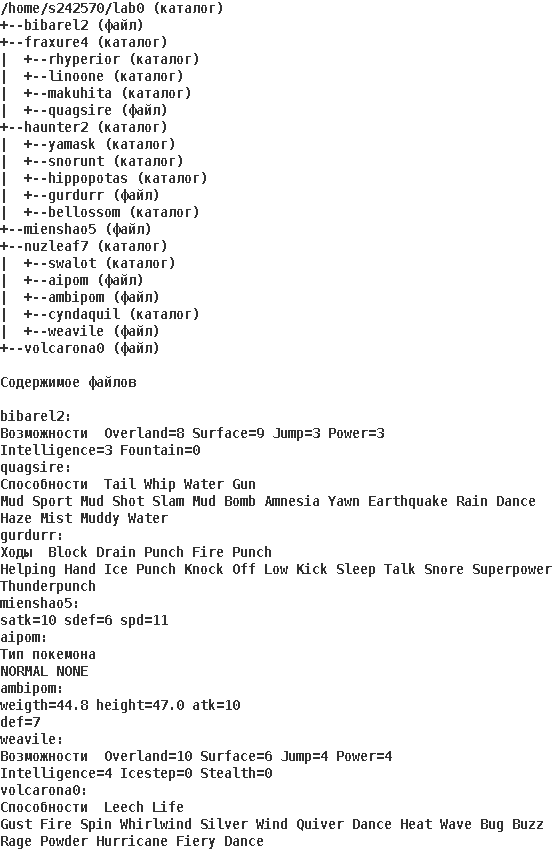
\includegraphics[width=250pt]{./1.png}
\small
\begin{enumerate}
\item Set up file and directory permissions chmod, using different approaches.
\begin{itemize}
\item bibarel2: rw--w-r--
\item fraxure4: rwxr-x-w--
\item rhyperior: владелец должен читать, записывать директорию и переходить в нее; группа-владелец должна читать, записывать директорию и переходить в нее; остальные пользователи должны читать, записывать директорию и переходить в нее-
\item linoone: права 337-
\item makuhita: владелец должен читать, записывать директорию и переходить в нее; группа-владелец должна записывать директорию и переходить в нее; остальные пользователи должны читать, записывать директорию и переходить в нее-
\item quagsire: ---rw--w--
\item haunter2: права 700-
\item yamask: владелец должен записывать директорию и переходить в нее; группа-владелец должна только переходить в директорию; остальные пользователи должны записывать директорию-
\item snorunt: r-xrwxrwx-
\item hippopotas: права 500-
\item gurdurr: права 640-
\item bellossom: права 511-
\item mienshao5: права 640-
\item nuzleaf7: владелец должен записывать директорию и переходить в нее; группа-владелец должна только переходить в директорию; остальные пользователи должны записывать директорию-
\item swalot: права 307-
\item aipom: ---r--r---
\item ambipom: владелец должен не иметь никаких прав; группа-владелец должна читать и записывать файл; остальные пользователи должны записывать файл-
\item cyndaquil: владелец должен читать директорию и переходить в нее; группа-владелец должна записывать директорию; остальные пользователи должны читать директорию-
\item weavile: права 064-
\item volcarona0: владелец должен не иметь никаких прав; группа-владелец должна читать и записывать файл; остальные пользователи должны записывать файл-
\end{itemize}
\item Copy tree parts and create links with cp and ln, as well as with cat and io streams redirection.
\begin{itemize}
\item скопировать рекурсивно директорию haunter2 в директорию lab0/fraxure4/rhyperior
\item создать символическую ссылку c именем Copy\(_{\text{52}}\) на директорию fraxure4 в каталоге lab0
\item cоздать символическую ссылку для файла mienshao5 с именем lab0/nuzleaf7/aipommienshao
\item объеденить содержимое файлов lab0/nuzleaf7/weavile, lab0/fraxure4/quagsire, в новый файл lab0/volcarona0\(_{\text{66}}\)
\item скопировать содержимое файла mienshao5 в новый файл lab0/haunter2/gurdurrmienshao
\item скопировать файл volcarona0 в директорию lab0/nuzleaf7/cyndaquil
\item cоздать жесткую ссылку для файла volcarona0 с именем lab0/nuzleaf7/weavilevolcarona
\end{itemize}
\item Using cat, wc, ls, head, tail, echo, sort, grep looks up and filters directory, files and data in it.
\begin{itemize}
\item Подсчитать количество строк содержимого файлов в директории nuzleaf7, отсортировать вывод по увеличению количества, ошибки доступа не подавлять и не перенаправлять
\item Вывести список имен и атрибутов файлов в директории fraxure4, список отсортировать по убыванию размера, подавить вывод ошибок доступа
\item Рекурсивно вывести содержимое файлов с номерами строк из директории lab0, имя которых начинается на 'a', строки отсортировать по имени a->z, ошибки доступа не подавлять и не перенаправлять
\item Подсчитать количество строк содержимого файла volcarona0, результат записать в тот-же файл, ошибки доступа перенаправить в файл в директории /tmp
\item Вывести три последних элемента рекурсивного списка имен и атрибутов файлов в директории lab0, содержащих строку "qu", список отсортировать по убыванию размера, подавить вывод ошибок доступа
\item Вывести содержимое файла mienshao5, строки отсортировать по имени a->z, добавить вывод ошибок доступа в стандартный поток вывода
\end{itemize}
\item Remove files using rm and rmdir according following:
\begin{itemize}
\item Удалить файл volcarona0
\item Удалить файл lab0/nuzleaf7/weavile
\item удалить символические ссылки Copy\(_{\text{*}}\)
\item удалить жесткие ссылки lab0/nuzleaf7/weavilevolcaro*
\item Удалить директорию nuzleaf7
\item Удалить директорию lab0/haunter2/hippopotas
\end{itemize}
\end{enumerate}
\end{document}